\newpage


%%%%%%%%%%%%%%%%%%%%%%%%%%%%%%%%%%%%%%%%%%%%%%%%%%%%%%%%%%%%%%%%%%%%%%%%%%%%%%%%%%%%%%%
%%%%%%%%%%%%%%%%%%%%%%%%%%%%%%%%%%%%%%%%%%%%%%%%%%%%%%%%%%%%%%%%%%%%%%%%%%%%%%%%%%%%%%%
%%%%%%%%%%%%%%%%%%%%%%%%%%%%%%%%%%%%%%%%%%%%%%%%%%%%%%%%%%%%%%%%%%%%%%%%%%%%%%%%%%%%%%%
\section{\textcolor{red}{Regressão logística-fourier e SE com classificador $f_{\VECTOR{c}}(\VECTOR{x}):~\mathbb{R}^{N} \rightarrow \mathbb{R}$}}
\label{sec:theo:reglogrnr1fourier:1}

\index{Regressão!Logística $f_{\VECTOR{c}}(\VECTOR{x}):~\mathbb{R}^{N} \rightarrow \mathbb{R}$}

\begin{theorem}[Classificação de dados em $\mathbb{R}$:]\label{theo:reglogrnr1fourier:1}
~\\
\noindent
\begin{minipage}{0.45\textwidth}
\centering
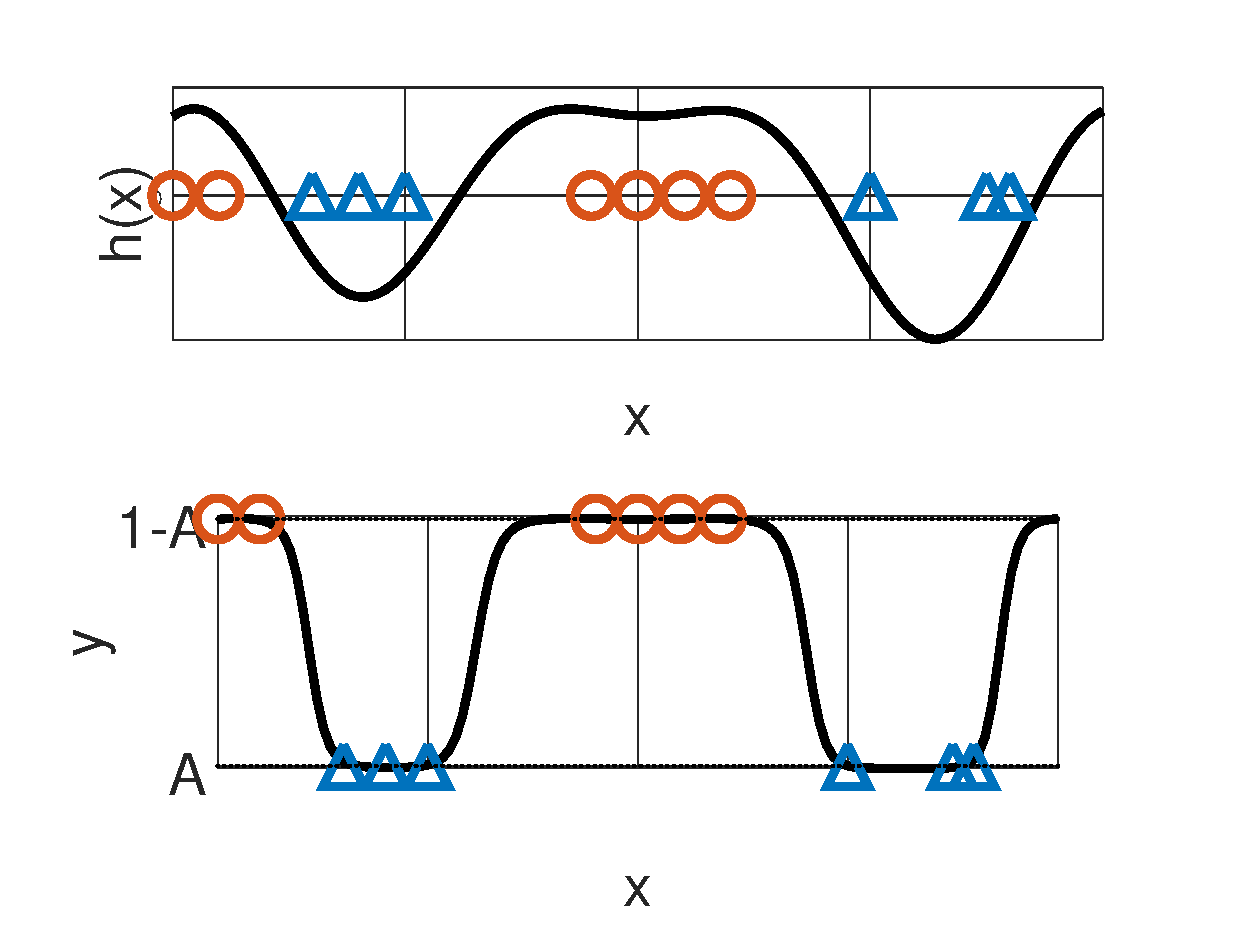
\includegraphics[width=0.95\linewidth]{chapters/classificacao/mfiles/reglogrnr1fourier/reglogrnr1fourier.eps} 
\end{minipage}
\begin{minipage}{0.55\textwidth}
Dados, um conjunto de $L$ pontos $\VECTOR{x}_l \in \mathbb{R}, 1 \leq l \leq L$,
repartidos em dois grupos etiquetados com os símbolos $\bigtriangleup$ e $\bigcirc$, 
e separáveis por um hiperplano.
Se desejamos criar um classificador mediante 
a função  $f_{\VECTOR{c}}:\mathbb{R}^{N} \rightarrow \mathbb{R}$,
com domínio $\VECTOR{x} \in \mathbb{R}^{N}$, contradomínio $y \in \mathbb{R}$ e 
parâmetros agrupados no vetor $\VECTOR{c}=[c_1~ c_2~ ...~ c_{{(2 K+1)}^N}]^{\transpose}\in \mathbb{R}^{2 K+1}$,
como definido na Eq. (\ref{eq:reglogrnr1fourier:1}),
\begin{equation}\label{eq:reglogrnr1fourier:1}
y\equiv f_{\VECTOR{c}}(\VECTOR{x})= \frac{1}{1+e^{-h_{\VECTOR{c}}(\VECTOR{x}) }},
\end{equation}
\end{minipage}
\begin{comment}
\begin{equation}
\begin{array}{lll}
 h_{\VECTOR{c}}(x) & = & 
        +\sum_{\VECTOR{k}=\VECTOR{0}}^{K} c_{2k} sin\left(k_1 \frac{2 \pi x_1}{L_1}\right)sin\left(k_2 \frac{2 \pi x_2}{L_2}\right) \\
~ & ~ & +\sum_{\VECTOR{k}=\VECTOR{0}}^{K} c_{2k} sin\left(k_1 \frac{2 \pi x_1}{L_1}\right)cos\left(k_2 \frac{2 \pi x_2}{L_2}\right) \\
~ & ~ & +\sum_{\VECTOR{k}=\VECTOR{0}}^{K} c_{2k} cos\left(k_1 \frac{2 \pi x_1}{L_1}\right)sin\left(k_2 \frac{2 \pi x_2}{L_2}\right) \\
~ & ~ & +\sum_{\VECTOR{k}=\VECTOR{0}}^{K} c_{2k} cos\left(k_1 \frac{2 \pi x_1}{L_1}\right)cos\left(k_2 \frac{2 \pi x_2}{L_2}\right).
\end{array}
\end{equation}
\end{comment}
\begin{equation}
 h_{\VECTOR{c}}(\VECTOR{x}) = 
\sum_{\VECTOR{k}=[-K,~ ...,-K]}^{[K,~ ...,K]}
c_{\VECTOR{k}}  e^{\mathbf{i}\VECTOR{k}^{\transpose}\MATRIX{W}_{\VECTOR{l}}\VECTOR{x}},
\quad
\MATRIX{W}_{\VECTOR{L}}=
\funcdiag\left(
\begin{bmatrix}
\frac{2 \pi}{l_1} &
\frac{2 \pi}{l_2} &
\dots &
\frac{2 \pi}{l_n} &
\dots &
\frac{2 \pi}{l_N}
\end{bmatrix}^{\transpose}
\right) 
\end{equation}

\textcolor{red}{Fingerprint a detectar surcos}\\
ou seu equivalente: $logit(y)=h_{\VECTOR{c}}(\VECTOR{x})$, onde\footnote{Tem 
que ser maior para evitar erros de $f_{\VECTOR{c}}(\VECTOR{x})$ nos extremos. 
Ex.: $L_x =1.1 || max(x_i)-min(x_i)||$.}
 $L_x > || max(x_i)-min(x_i)||$.

Podemos atribuir a cada valor $\VECTOR{x}_l$ uma etiqueta $y_l\in \{A,1-A\}$, 
onde $0<A\ll 0.5$ é escolhido por nós,
e afirmar que o vetor $\VECTOR{c}= \VECTOR{\hat{c}}$,
que minimiza o erro quadrático $e(\VECTOR{c})$,
\begin{equation}\label{eq:reglogrnr1fourier:1e}
e(\VECTOR{c}) =  \sum_{l=1}^{L} q_l||h_{\VECTOR{c}}(\VECTOR{x}_l) -logit(y_l)||^2,
\end{equation}
ponderado usando os pesos $q_l \in \mathbb{R}_+$, 
pode ser achado\footnote{A demostração pode ser vista na Prova \ref{proof:theo:reglogrnr1fourier}.}  
com
\begin{equation}\label{eq:reglogrnr1fourier:2}
\VECTOR{\hat{c}} =  \left[ \MATRIX{A}^{\transpose} \MATRIX{Q}\MATRIX{A}\right]^{-1} \MATRIX{A}^{\transpose} \MATRIX{Q}\VECTOR{z},
\quad
\MATRIX{A}=
\begin{bmatrix}
\VECTOR{a}_{K}(\VECTOR{x}_1) \\
\VECTOR{a}_{K}(\VECTOR{x}_2) \\
\vdots \\
\VECTOR{a}_{K}(\VECTOR{x}_l) \\
\vdots \\
\VECTOR{a}_{K}(\VECTOR{x}_L) \\
\end{bmatrix},
\quad
\MATRIX{Q}=\funcdiag \left(
\begin{bmatrix}
q_1  \\
q_2  \\
\vdots  \\
q_l  \\
\vdots \\
q_L \\
\end{bmatrix}
\right),
\quad
\VECTOR{z}=
\begin{bmatrix}
logit(y_1)  \\
logit(y_2)  \\
\vdots  \\
logit(y_l)  \\
\vdots \\
logit(y_L) \\
\end{bmatrix},
\end{equation}
\begin{equation}
\VECTOR{a}_{K}(\VECTOR{x})=
\begin{bmatrix}
\frac{1}{2} & %\VECTOR{b}_{0}(\VECTOR{x}) &
\VECTOR{b}_{1}(\VECTOR{x}) &
\dots  &
\VECTOR{b}_{k}(\VECTOR{x}) &
\dots  &
\VECTOR{b}_{K}(\VECTOR{x})
\end{bmatrix}.
\end{equation}
\end{theorem}
\begin{tcbattention}
\begin{itemize}
\item Dado que a função de classificação $f_{\VECTOR{c}}(\VECTOR{x})$ vai entre $0$ e $1$,
podemos reinterpretar este valor como se fosse uma probabilidade;
neste caso, $f_{\VECTOR{c}}(\VECTOR{x})$ representa a probabilidade de que um valor $\VECTOR{x}$
pertença ao grupo $\bigcirc$.
\item O limiar da classificação de $f_{\VECTOR{c}}(\VECTOR{x})$ 
está no hiperplano $h_{\VECTOR{c}}(\VECTOR{x})=0$,
provocando neste ponto um $f_{\VECTOR{c}}(\VECTOR{x})=0.5$.
\item $L_x$ indica o periodo de repetição do classificador,
por este motivo o classificador é interessante quando o domínio dos dados ($\VECTOR{x}_l$) está restrito.
\end{itemize}
\end{tcbattention}

